\chapter{Compiler technology as a mediator between OOP and DoD}
The inherent purpose of a compiler is to read a program defined in a \textit{source language} and translate it to an equivalent pendant for a \textit{target language} \mcp{aho}{1}. They are yet another form of abstraction, that enable us to work more efficiently. Low-level languages interact 'less indirectly' with the hardware (more control) thus enable one to write better performing code. But they are usually harder to write as well as less portable, more prone to errors, and harder to maintain \mcp{aho}{17}.\\
Compilers provide some of the most important features a programmer needs, like syntactic and semantic analysis steps, which can automate the process of finding errors and even just smelly code. To do that they need some sort of 'understand' for the program.

\section{A compiler's understanding of the program}\label{compilers_understanding}
\begin{wrapfigure}[8]{r}{0.4\textwidth}
	\begin{lstlisting}[numbers=none, name={Exerpt of example context free grammar defining a (if)statement. Bold = terminal; italic = nonterminal}, emph={stmt, optexpr}, emphstyle=\itshape, morekeywords={expr, if}, mathescape=true, literate={->}{$\rightarrow{}$}{1}, label={bnf}]
	stmt -> expr ;
	| if ( expr ) stmt
	\end{lstlisting}
\end{wrapfigure}
Modern compilers implement several \textit{phases} bundled in \textit{passes} to provide an abstraction rich routine from reading mere character sequences until generating char sequences in the target language \reffigp{compiler_phases}. Of course compilers are not thinking entities, but there are mechanisms to formally define a language as well as steps to generate semantic statements with it, ordering them in a way so that a computer can process them in a meaningful way.
\subsubsection{Syntax definition}
\begin{wrapfigure}[8]{l}{0.32\textwidth}
	\begin{center}
		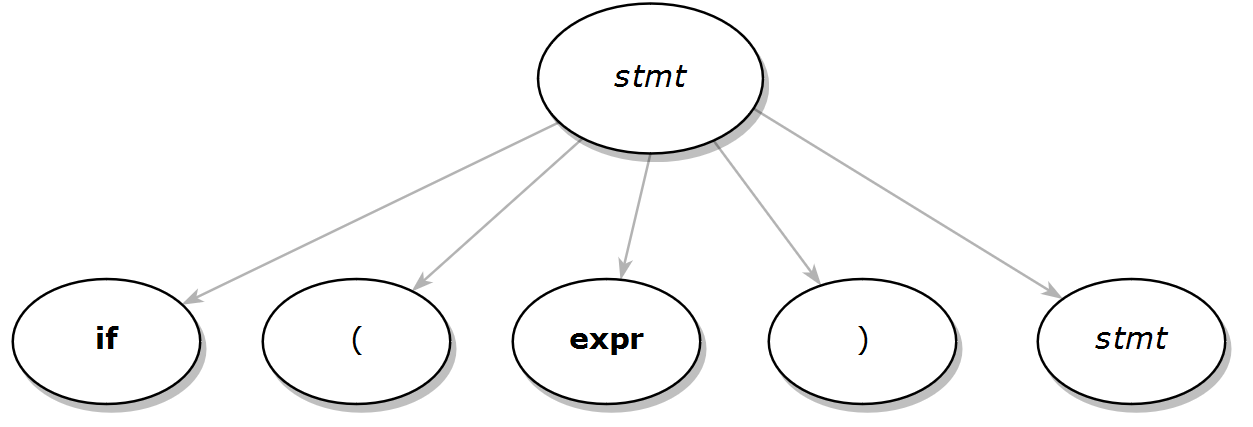
\includegraphics[width=.32\textwidth, height=0.12\textheight]{PICs/parse_tree}
	\end{center}
	\caption{Parse tree for the if-stmt node.}\label{parse_tree}
\end{wrapfigure}
A syntactical language definition can be done using the \textit{context free grammar} notation or \textit{BNF} (Backus-Naur Form) \mcp{aho}{40}. Those grammars define a hierarchy of rules on how to form statements/expressions in the language. By defining a set of elementary symbols (\textit{terminals}) for example keywords we can then define more complex \textit{nonterminals}, like defining how a statement is formed. Ultimately we can make \textit{production} rules that describe for example our control flow statements \refcodep{bnf}. Just like this set of grammar rules basically constitutes a hierarchy we can deduce a \textit{parse tree} for it as a concrete implementation, where beginning from the start symbol we can derive valid successors for each symbol by iterating its child nodes. Given a statement like: "$\textit{\textbf{if} \textbf{true}) i++;}$". After reading the first token \textit{if} we can iterate our parse tree's production node for that statement and easily see, that the rule demands an opening bracket immediately following the if terminal, rendering the input as syntactically ill-formed \reffigp{parse_tree}. To be able to analyze a program like this we initially need to pass through a few \textit{phases} transforming and collecting data until we have a representation, we can work with.

\subsubsection{Lexical analysis}
\begin{wrapfigure}[20]{r}{0.2\textwidth}
	\begin{center}
		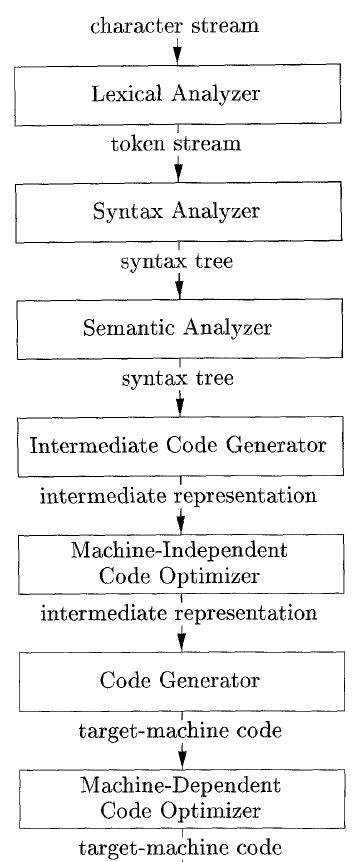
\includegraphics[width=.3\textwidth, height=0.45\textheight]{PICs/compiler_phases}
	\end{center}
	\caption{Phases of a compiler \mcppic{aho}{5}.}\label{compiler_phases}
\end{wrapfigure}
The compilers \textit{Lexer} or \textit{Scanner} takes the raw sequence of chars forming the source code and creates tokens out of char subsets it identifies as such. This information is used to fill the \textit{Symbol table}, which holds information like types, relative positions of the values, scopes and more. The symbol table is used in several following phases and essential for correct linkage of different compilation units.
\subsubsection{Syntax analysis}
The syntax analyzer creates the first \textit{Intermediate Representation} of the source code, the \textit{Syntax Tree} or \textit{Abstract Syntax Tree} (AST). It takes the token stream provided by the first phase and orders them in a tree like structure that already accounts for computational order and depicts the the grammar of the input.
\subsubsection{Semantic analysis}
Analyzing the AST from the previous phase is the \textit{Semantic Analyzer}'s duty. It traverses the AST and constantly compares its nodes with the formal language definition and gathers information like type traits. Consequently \textit{type checking} - which is important for statically typed languages - will take place in this phase \mcp{aho}{5-9}.

\section{A useful interface}
As can be seen in \reffig{compiler_phases} there are several more phases left to describe, however \refsec{compilers_understanding} already provides information that we can utilize towards implementing a tool, that automatically translates OOP code into a cache friendly pendant.\\
Assuming we have access to our programs AST, we could start analyzing the code in an environment, that allows us to traverse the code in a tree like fashion. This means easy access to the defined data layout, as well as the access patterns in use.\\
Luckily modern compilers are designed in a modular fashion and usually define \textit{front ends} and \textit{back ends} to facilitate a multiple language to machine mapping. The front end consists of the analysis phases as well as the intermediate code generation phases for a source language. After generating an immediate representation (IR) it is forwarded to the back end which \textit{synthesizes} the end product in the desired target language \mcp{aho}{4}.\\
The front end is especially interesting to us since it provides us with the appropriate representations to thoroughly investigate a program. 

\subsubsection{LLVM/Clang}
A rather prominent representative of such an assembler/compiler/debugger tool-chain is the open source LLVM project. The front end functionality for C++ is here implemented in the Clang compiler. All the functionality is accessible and furthermore served through diverse libraries and interfaces - for example the \textit{LibTooling} library that brings functionality for parsing code, creating ASTs and running \textit{FrontEndActions} over it. There are already mechanisms for recursive AST traversal like \textit{Recursive AST Visitors} and AST matching functionality with the \textit{AST Matchers}. Also tools like \textit{clang-query} provide a \textit{REPL} (Read-Eval-Print Loop) environment for quick testing.





